\subsection{UML2-Komponentendiagramm}

\begin{figure}[H]
    \centering
    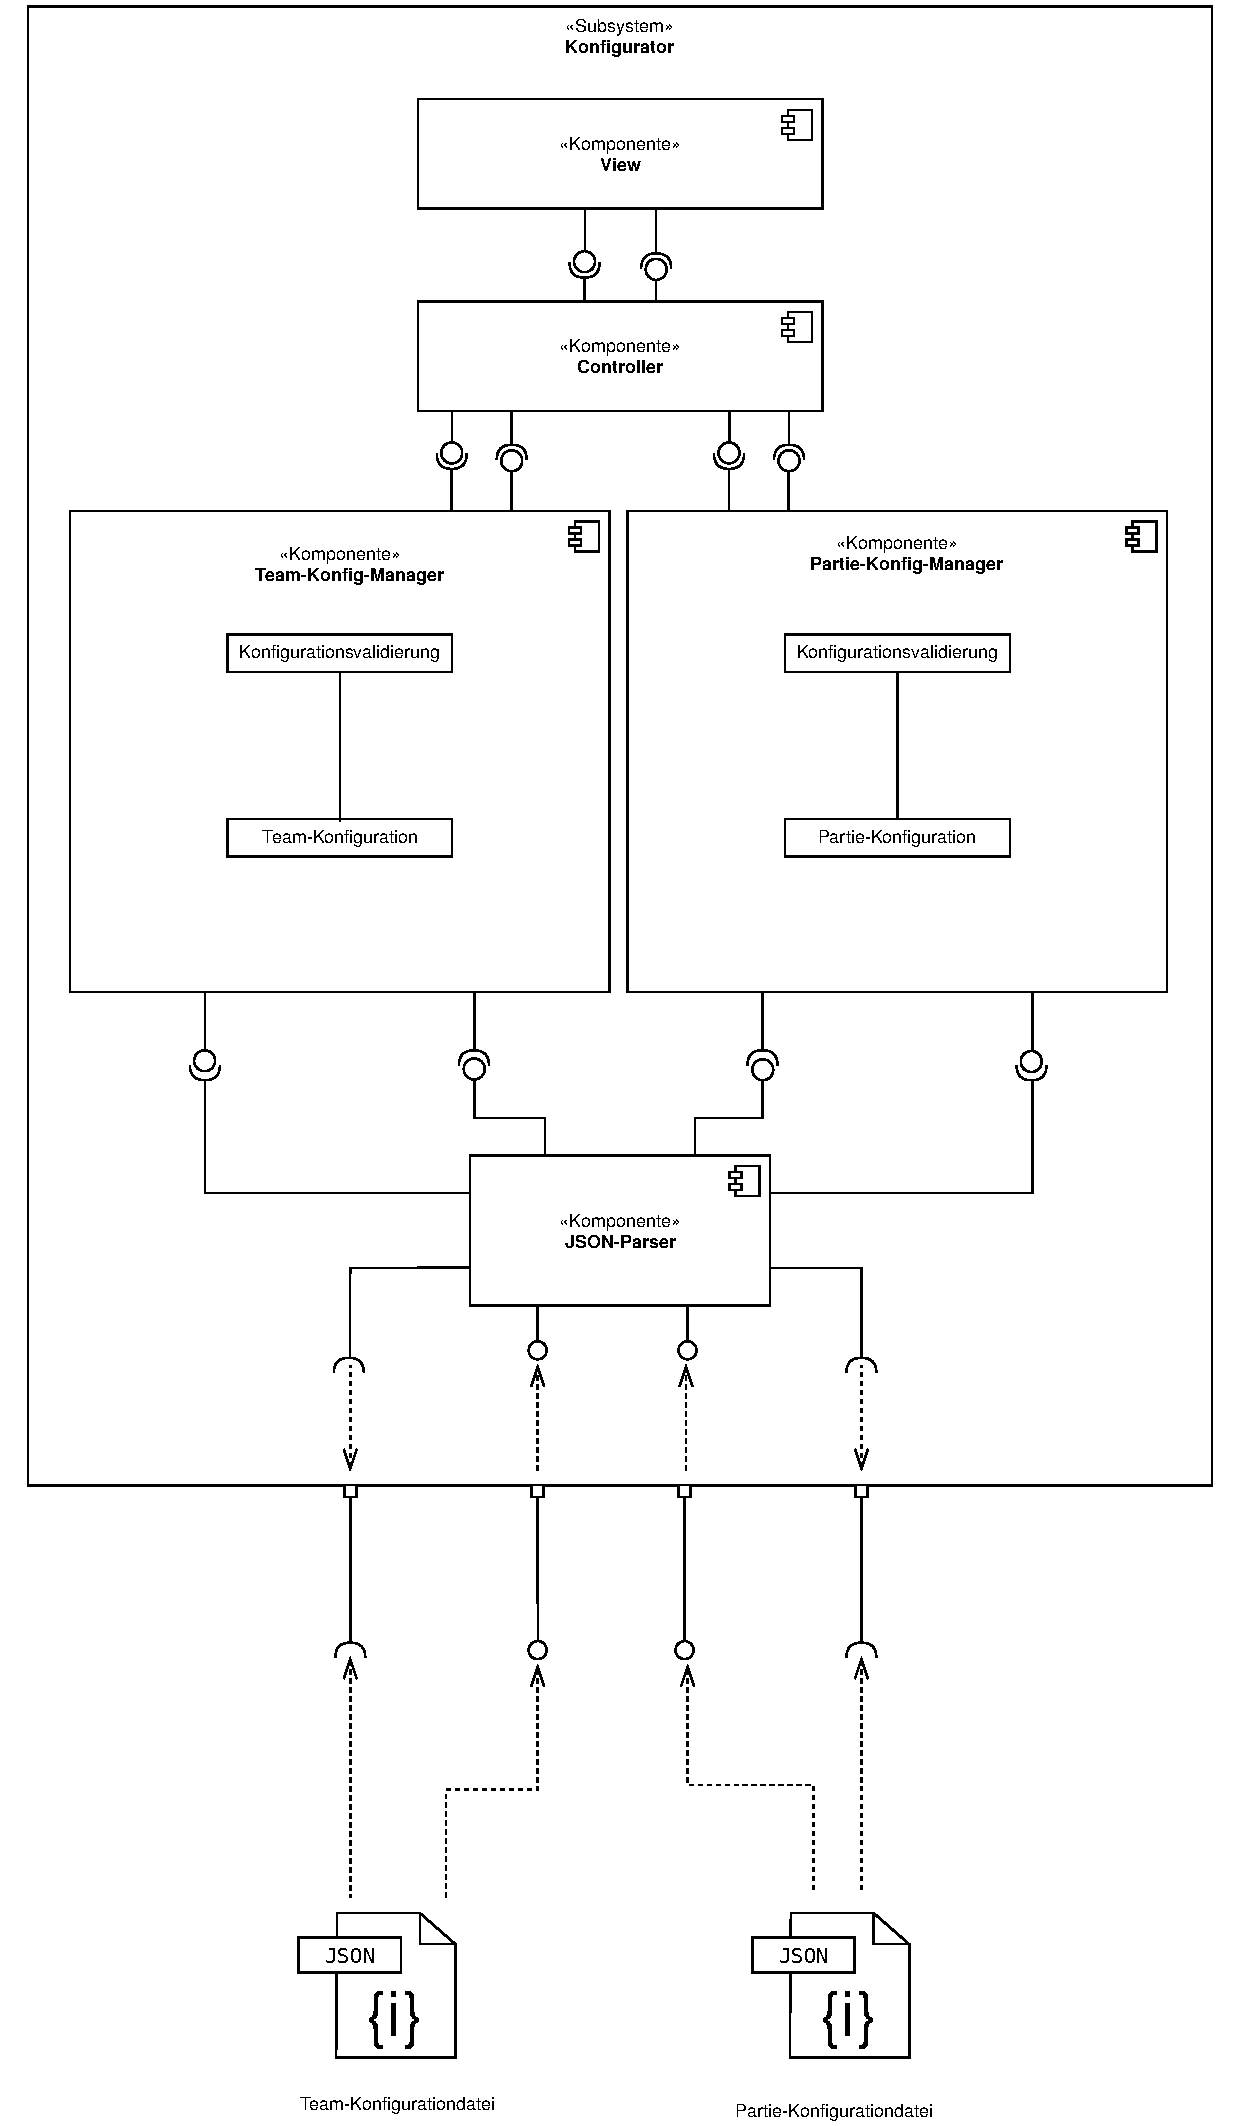
\includegraphics[scale=0.6]{images/Konfigurator.pdf}
\end{figure}

\subsection{Beschreibungen}

\begin{description}

\item[Konfigurator]

Beim Subsystem Konfigurator handelt es sich um eine graphische Benutzeroberfläche, die der Erstellung von Partie- oder Team-Konfigurationen dient. Der Konfigurator ist ein eigenes Programm, und somit unabhängig von den anderen Anwendungen.

\item[Team-Konfig-Manager]
Der Team-Konfig-Manager verwaltet eine Team-Konfiguration. Er kommuniziert über den Controller mit der View und nimmt ebenfalls neue Daten von dieser entgegen. Bevor die Daten, die der Nutzer in der graphischen Oberfläche einstellt, in einem Team-Konfigurations-Objekt gespeichert werden, werden sie zuvor noch von der Konfigurationsvalidierung überprüft, sodass sichergestellt ist, dass nur gültige Konfigurationen erstellt werden können. Der Team-Konfig-Manager kümmert sich nur um die programminterne Repräsentation der Konfiguration und ist deshalb streng von der Anzeige sowie dem JSON-Parser getrennt.

\item[Partie-Konfig-Manager]
Der Team-Konfig-Manager verhält sich analog zum Team-Konfig-Manager. Er unterscheidet sich lediglich in der Konfigurationsvalidierung, die natürlich auf eine ebenfalls unterschiedliche Repräsentation der Konfiguration zugeschnitten ist.

\item[Team-Konfi-Manager]
Der Controller kümmert sich streng nach dem MVC-Pattern um die Kommunikation zwischen den Konfig-Managern un der graphischen Anzeige. Änderungen des Nutzers in der GUI werden an den passenden Konfig-Manager weitergegeben und andersherum erhält die GUI über den Controller immer den aktuellsten Zustand der Konfiguration.
\item[JSON-Parser]
Der JSON-Parser serialisiert bzw. deserialisiert die Konfigurationen, um sie zu speichern, bzw. zu laden. Er erhäkt von den Konfig-Managern ein Konfigurationsobjekt und serialisiert dieses, damit es im Filesystem gespeichert werden kann oder lädt eine Konfiguration aus einer Datei und gibt sie an den passenden Konfig-Manager weiter.
\end{description}

\subsection{Zuordnung der Funktionalen Anforderungen}

Die funktionalen Anforderungen gemäß dem Pflichtenheft werden den Komponenten folgendermaßen zugeteilt:

\begin{table}[h]
    \centering
    \begin{tabular}{|l|l|}
        \hline
        \textbf{Komponente} & \textbf{Abgedeckte funktionale Anforderungen}\\ \hline
        Team-Konfiguration & FA53, FA70 \\ \hline

        Partie-Konfiguration & FA54, FA70 \\ \hline

        JSON-Konverter & FA71, FA72 \\ \hline


    \end{tabular}
\end{table}
